\documentclass[11pt,a4paper,english]{article}

\usepackage{hyperref}
\usepackage{multicol}
\usepackage{array}
\usepackage{url}
\usepackage{amsmath}
\usepackage{amssymb}
\usepackage{subfig}
\usepackage[english]{babel}
\usepackage{blindtext}
\usepackage{graphicx}
\usepackage{todonotes}
\usepackage{tikz}
\usepackage[section]{placeins}
\usepackage{afterpage}
\usetikzlibrary{arrows,positioning}
%\usepackage[disable]{todonotes}
\usepackage[a4paper, bottom=38mm, footskip=30mm]{geometry}


%%% Header and footer style
% TODO: improve header/footer styles
\usepackage{fancyhdr}
\pagestyle{fancy}
\fancyhf{}
\fancyhead[LE,RO]{\bfseries\thepage}
\fancyhead[LO]{\bfseries\rightmark}
\fancyhead[RE]{\bfseries\leftmark}
\renewcommand{\headrulewidth}{0.5pt}
\addtolength{\headheight}{0.5pt}
\fancypagestyle{plain}{%
   \fancyhf{}
   \fancyfoot[C]{\bfseries \thepage}
   \fancyhead{}%get rid of headers on plain pages
   \renewcommand{\headrulewidth}{0pt} % an the line
}

% title page config
\newcommand{\sctTitle}{Interfacing TVLA and Sample}
\newcommand{\sctAuthor}{Raphael Fuchs}
\newcommand{\sctSupervisor}{Dr. Pietro Ferrara}
\newcommand{\sctReportType}{Bachelor Thesis Report}
\newcommand{\sctDate}{\today}
\newcommand{\sctKeywords}{Shape Analysis TVLA Sample Static Analysis}


% enumeration formats
\renewcommand\theenumi{\arabic{enumi}}
\renewcommand\labelenumi{\theenumi.}
\renewcommand\theenumii{\roman{enumii}}
\renewcommand\labelenumii{\theenumii)}

% dont indent paragraphs 
\usepackage[parfill]{parskip}


%%% hyperlinks
\hypersetup{%
   pagebackref=true,
   colorlinks=true,
   bookmarks=true,
   bookmarksopen=false,
   bookmarksnumbered=true,
   pdftitle={\sctTitle},
   pdfauthor={\sctAuthor},
   pdfkeywords={\sctKeywords ETH Zurich Computer Science}
}


\usepackage{listings}

% Scala language definition
\lstdefinelanguage{scala}{
  morekeywords={abstract,case,catch,class,def,%
    do,else,extends,false,final,finally,%
    for,if,implicit,import,match,mixin,%
    new,null,object,override,package,%
    private,protected,requires,return,sealed,%
    super,this,throw,trait,true,try,%
    type,val,var,while,with,yield},
  otherkeywords={=>,<-,<\%,<:,>:,\#,@},
  sensitive=true,
  morecomment=[l]{//},
  morecomment=[n]{/*}{*/},
  morestring=[b]",
  morestring=[b]',
  morestring=[b]"""
}

% listing format for TVP
\lstdefinelanguage{tvp}{
  morekeywords={foreach, in, E,unique,function,nonabs},
  otherkeywords={\%\%,\%action,\%f,\%p,\%s},
  sensitive=true,
  morecomment=[l]{//},
  morecomment=[n]{/*}{*/},
  morestring=[b]",
  morestring=[b]',
  morestring=[b]"""
}

% listing format for TVS
\lstdefinelanguage{tvs}{
  morekeywords={},
  otherkeywords={\%n,\%p,->,:},
  sensitive=true,
  morecomment=[l]{//},
  morecomment=[n]{/*}{*/},
  morestring=[b]",
  morestring=[b]',
  morestring=[b]"""
}

\definecolor{dkgreen}{rgb}{0,0.6,0}
\definecolor{gray}{rgb}{0.5,0.5,0.5}
\definecolor{mauve}{rgb}{0.58,0,0.82}
	
% default listing format (Scala!)
\lstset{frame=tb,
  language=scala,
  aboveskip=3mm,
  belowskip=3mm,
  showstringspaces=false,
  columns=fixed,
  basicstyle={\small\ttfamily},
  numbers=left,
  numberstyle=\tiny\color{gray},
  keywordstyle=\color{blue},
  commentstyle=\color{dkgreen},
  stringstyle=\color{mauve},
  frame=single,
  breaklines=true,
  breakatwhitespace=true,
  tabsize=3,
  captionpos=b,
  numberbychapter=true
}



% FONTS
\usepackage{fontspec}
\usepackage{xcolor}
\usepackage{xunicode}
\usepackage{xltxtra}
\defaultfontfeatures{Mapping=tex-text}
\setromanfont{Palatino LT Std}
\setmonofont[Scale=0.85]{Luxi Mono}
\definecolor{HeadingColor}{HTML}{00335b}
\newfontfamily\titlefont[Color=HeadingColor]{Linux Libertine}

% TikZ heap graph styles
\tikzset{
  every node/.style={on grid,node distance=2cm and 2cm},
  hid/.style={circle,draw=blue!80,fill=blue!30,thick,minimum size=1cm},
  nn/.style={minimum size=1cm},
  sum/.style={circle,draw=black!80,fill=blue!30,thick,minimum size=1cm,dashed},
  var/.style={rectangle,draw=black,fill=black!20,thick,minimum size=0.6cm},
  %edge styles
  every edge/.style={->,draw=black,thick,>=latex}
}

% custom autoref names
\def\subsubsectionautorefname{Section}
\def\subsectionautorefname{Section}
\def\subfigureautorefname{Figure}
\def\sectionautorefname{Section}


% boxes for listings as subfigures
\newsavebox{\mylistingbox}
\newsavebox{\mygraphboxA}
\newsavebox{\mygraphboxB}
\newsavebox{\mygraphboxC}

% remove??
\afterpage{\clearpage}

\newcommand{\makecustomtitlepage}{
\thispagestyle{empty}

{

\vspace*{\fill}
\vspace*{\fill}

\begin{center}
\textsc{\huge \color{HeadingColor}
\titlefont\sctTitle
}

\vspace{\fill}

{\Large \sctAuthor}

\vspace{\fill}

{\Large \sctReportType}

\vspace{\fill}

{\Large Chair of Programming Methodology} \\
{\Large Department of Computer Science} \\
{\Large ETH Zurich}\\[5mm]
%{\Large \url{http://www.pm.inf.ethz.ch/}}

\vspace{\fill}

{\Large \sctDate}

\end{center}

\vspace{\fill}
\noindent
\textbf{Supervised by:} \\
\hspace*{1cm} \sctSupervisor \\
\hspace*{1cm} Prof.~Dr.~Peter~M\"{u}ller \\


\vspace{\fill}

%\hspace{-2cm}
\noindent
\begin{minipage}[b]{10cm}
\textbf{\large Chair of Programming Methodology}\\

\includegraphics[width=3cm]{img/inf-logo}
\end{minipage}
\hfill

\includegraphics[width=4.5cm]{img/ethlogo_black}

}

\newpage
}

\begin{document}
\makecustomtitlepage

\begin{abstract}
In this bachelor thesis we plug shape analysis into the generic static analyzer
Sample, providing an interface to the tool TVLA. Our approach integrates the new
domain with the existing semantic domains such that other information about the
content of heap locations can be combined with TVLA. 

\end{abstract}
\thispagestyle{empty}
\newpage


\tableofcontents
\newpage

\section{Introduction}
\subsection{Overview}
The goal of this thesis is to enhance the static analyzer Sample with
\textit{shape analysis} capabilities by interfacing it with TVLA. In this
introduction, we briefly present the motivation of our work as well as a brief 
description of TVLA and Sample.

\subsection{Shape Analysis: Motivation}
Shape analysis is concerned with statically and automatically inferring
properties about the heap of a program, also called store. A state of
the program heap can be thought of as a graph where the nodes represent blocks
of allocated memory and the edges pointers between those blocks, together with a
set of program variables (called the environment) which may also point to heap
nodes.

One possible question is about the reachability of heap
nodes. Given two nodes and starting from the first one, is it possible to reach
the second one by following pointers? Other important properties include cyclicity,
sharing, may-aliasing and disjointness \cite{wilhelm2000shape}.  More generally,
one may be interested in the ``shape'' of a heap, that is a characterization of
its data structures. For a program which manipulates singly linked lists, this
would mean that we could statically determine that its heap contains lists, and
also whether they contain cycles or not. Other common data structures of
interest include doubly linked lists, trees and DAGs.

The results of a shape analysis have many applications. They are helpful or even
necessary for certain forms of program verification (e.g. freedom from
null-pointer dereferences), optimization and automatic parallelization (disjoint
data structures may be processed in parallel) etc.

Unfortunately, one can not give precise answers to all of the above questions
for all possible programs. It is well-known that many interesting properties
such as program termination are undecidable. Even decidable properties are often
too expensive to be analyzed as the problem at hand suffers from state space
explosion. Therefore we need to introduce approximation: The program semantics is
approximated so that the answer is not wrong but less precise. Roughly, if we
prove a property on the approximation, then this property is respected by all
possible executions. Instead, if the property is not proven, this could be a
false alarm because of a too rough approximation.

In the case of heap analysis, we often have programs that manipulate
structures of unbounded size. For example, the length of lists is unbounded.
However, we need a bounded representation in our analysis.  This usually implies
the need for a conservative approximation.

Heap abstraction has proven to be a particularly hard problem in static
analysis. During the last decade, TVLA has been

\subsection{TVLA} 
\textit{Parametric shape analysis via 3-valued logic} is a technique introduced
by Sagiv et al.  \cite{sagiv2002parametric} and to date remains the most
promising approach to heap analysis. Lev-Ami implemented these ideas in a tool
called TVLA (Three-valued Logic Analysis Engine) \cite{lev2000tvla}, which we
are going to use in this thesis.

In the following, we outline some of the ideas behind this static
analysis and how the theoretical concepts translate to TVLA. We try to keep the
explanation general and focused on the logic for now. 

\subsubsection{Representing Concrete Heaps}
\label{sct:structDef}
Heaps in TVLA are represented using logical structures. A structure $S$
consists of a tuple $(U^S,I^S)$ where $U^S$ is the universe with elements called
\textit{individuals} and $I^S$ is an interpretation of a \textit{vocabulary} of
predicate symbols over $U^S$.

A structure describes a particular instance of the heap: We can interpret the
individuals to be the set of nodes in the heap graph, i.e. the set of allocated
memory blocks. The valuation of the predicates encodes all the information that
makes up the heap. \textit{Unary predicates} can for instance encode that a
program variable points to a heap node: If variable $x$ references node $n1$, we
create a unary predicate $x$ such that $x(n1) = 1$. \textit{Binary predicates} on the
other hand can express which objects a field references (defining the edges
between nodes if the heap is thought to be a graph).

\textit{Example: } \autoref{fig:exampleConcrete} shows our running example with
a structure that consists of three heap nodes as it is encoded in the TVS format
used by TVLA. We see that the unary predicate \texttt{x} holds for \texttt{n1},
i.e. $x(n1) = 1$, and \texttt{n1} is related to \texttt{n2} by the binary
predicate \texttt{f}, i.e.  $f(n1,n2) = 1$.

\begin{figure}[h]
  \begin{lrbox}{\mylistingbox}
\begin{minipage}[b]{.45\linewidth}
\begin{lstlisting}[boxpos=b,language=tvs,label=lst:exampleConcrete]
// individuals
%n = {n1, n2, n3}
// interpretation of predicates
%p = {  
  x = {n1}
  f = {n1 -> n2, n2 -> n3}
}
\end{lstlisting}
\end{minipage}
  \end{lrbox}
  \subfloat[TVS Encoding]{\usebox{\mylistingbox}}
  \hspace{1cm}
  \subfloat[Visualization]{%
    \begin{tikzpicture}
    \node[hid] (n1) {n1};
    \node[var] (x) [above=of n1] {x}
      edge [->] (n1);
      
    \node[hid] (n2) [right=of n1] {n2}
      edge[<-] node[auto,swap] {f} (n1);
    \node[hid] (n3) [right=of n2] {n3}
      edge[<-] node[auto,swap] {f} (n2);
  \end{tikzpicture}}
  \caption{A 2-valued Heap Structure}
  \label{fig:exampleConcrete}
\end{figure}
To extract information from such a heap, one may simply evaluate a formula of
first-order logic (with transitive closure) over the structure.

\subsubsection{Heap Abstraction} 
Instead of 2-valued logical structures, Kleene's 3-valued logic is used to
describe abstract heaps with 3-valued structures: In addition to 'true' and
'false', there is a third 'unknown' (also written $1/2$) truth value.  

When considered 'equivalent` in some sense, several heap nodes can be combined into a
single one, called a summary node, representing one or more concrete nodes. A
given 3-valued structure can (conservatively) represent infinitely many concrete
ones.

The decision when to apply summarization is based on the notion of
\textit{canonical abstraction}: All nodes that agree on the values of a chosen
set of unary \textit{abstraction predicates} are considered to be equivalent and
therefore mapped to the same individual in the output structure.

\begin{figure}[h]
\begin{lrbox}{\mylistingbox}
\begin{minipage}[b]{.45\linewidth}
\begin{lstlisting}[boxpos=b,language=tvs]
// individuals
%n = {n1, n2} 
// interpretation of predicates
%p = { x = {n1}
  f = {n1 -> n2, n2 -> n2: 1/2}
  sm = {n2: 1/2} // n2 is summarized
}
\end{lstlisting}
\end{minipage}
  \end{lrbox}
  \subfloat[TVS Encoding]{\usebox{\mylistingbox}}
  \hspace{1cm}
  \subfloat[Visualization]{\begin{tikzpicture}
    \node[hid] (n1) {n1};
    \node[var] (x) [above=of n1] {x}
      edge [->] (n1);
      
    \node[sum] (n2) [right=of n1] {n2}
    edge[<-,dashed] node[auto] {f} (n1)
    edge[->,dashed,loop] node[auto,swap] {f} (n2);
  \end{tikzpicture}}
  \caption{Abstracted Structure (3-valued)}
  \label{fig:exampleAbstract}
\end{figure}

\textit{Example: } \autoref{fig:exampleAbstract} displays the same structure as
in the previous example, but this time after abstraction was applied (with
\texttt{x} as abstraction predicate). Since $x(n2) = x(n3) = 0$ in the original
structure, $n1$ and $n2$ were summarized in the 3-valued structure.


\subsubsection{Expressing Semantics and Programs}
In TVLA, the semantics of statements are defined by \textit{actions}. Actions
can take parameters and describe how to transform a given state into a new one
using predicate logic. In particular, this is done using a set of \textit{predicate-update
formulae}. For each predicate in the vocabulary, a logical formula, the update
predicate, specifies the new interpretation in terms of the pre-state.

As input, a TVP (Three-Valued Program) file declares the
predicates used, the available actions, and specifies a control flow graph where
the edges are instantiations of the actions.

\textit{Example: } Let the abstract heap in \autoref{fig:exampleAbstract} be our
pre-state and assume we  want to set the $f$-field of node $n1$ to
\texttt{null}. In a programming language this could be expressed as \texttt{x.n
= null}. To encode this as TVP, we introduce a general action
\texttt{setFieldNull(c,n)} which can be used to set a particular field of a node
pointed by a program variable to \texttt{null}. We then instantiate this action
with $x$ (to denote $n1$) and our field predicate $f$ as parameter.
\autoref{lst:tvp} shows the complete TVP and \autoref{fig:tvpResult} displays
the resulting abstract heap after TVLA was invoked.

\begin{lstlisting}[language=tvp,caption={TVP for Example},label=lst:tvp]
// predicate declaration
%p x(v_1) unique
%p f(v_1,v_2) function
%%
// action declaration
%action setFieldNull(c,n) {
	{ n(v_1,v_2) = n(v_1,v_2) & !c(v_1) }
}
%%
// control flow graph
start setNextNull(x,f) end
\end{lstlisting}

\begin{figure}[h]
\begin{lrbox}{\mylistingbox}
\begin{minipage}[b]{.45\linewidth}
\begin{lstlisting}[boxpos=b,language=tvs]
// individuals
%n = {n1, n2} 
// interpretation of predicates
%p = { x = {n1}
  f = {n2 -> n2: 1/2}
  sm = {n2: 1/2} // n2 is summarized
}
\end{lstlisting}
\end{minipage}
  \end{lrbox}
  \subfloat[TVS Encoding]{\usebox{\mylistingbox}}
  \hspace{1cm}
  \subfloat[Visualization]{\begin{tikzpicture}
    \node[hid] (n1) {n1};
    \node[var] (x) [above=of n1] {x}
      edge [->] (n1);
      
    \node[sum] (n2) [right=of n1] {n2}
    edge[->,dashed,loop] node[auto,swap] {f} (n2);
  \end{tikzpicture}}
  \caption{Result after Execution}
  \label{fig:tvpResult}
\end{figure}

  
\subsubsection{Refining the Abstraction}  
To improve the precision of the analysis, \textit{instrumentation predicates}
can be added. They express properties of interest in terms of basic \textit{core
predicates}. They often lead to finer distinctions among the concrete structures
represented by the abstract heap and can be used to tune the shape analysis for
certain data structures.

Summary nodes can also be split into separate nodes again in a process
called \textit{materialization}: Certain 'unknown' (1/2) values in the heap
structures may be forced to take on definite ('true'/'false') truth values.
\textit{Focus formulas} are used to characterize the parts of the heap that need to
assume definite values, i.e. that we are focusing on. 

Finally, \textit{integrity constraints} (also called compatibility constraints)
ensure that the abstracted structures satisfy some consistency rules (e.g.
global invariants). Sometimes, a 3-valued structure created does represent any
legal concrete structure and may therefore be dropped.

\textit{Example: } Consider our running example again. Assume we start with the
abstract state depicted in \autoref{fig:exampleAbstract} and want to access the
node that the first node $n1$ references with its field $f$, i.e. to execute
\texttt{p = x.f}. The resulting heap structures are shown in
\autoref{fig:noReach}. In the first and second structure we see that a node was
successfully materialized out of the summary node again and now referenced by
$p$. The information how many nodes there were exactly in the original structure
is lost as part of the abstraction. However, this failed for the third structure
 c: The abstraction also did not preserve the fact whether
the concrete nodes represented by $n2$ are actually reachable from $n1$.
Therefore, the case where this is not the case  was also considered.  We can
improve the analysis and eliminate this case by adding an instrumentation
predicate for reachability.
\begin{figure}
  \begin{center}
  \begin{lrbox}{\mygraphboxA}
    \begin{tikzpicture}
    \node[hid] (n1) {n1};
    \node[var] (x) [above=2cm of n1] {x}
      edge [->] (n1);
    \node[sum] (n2) [right=2cm of n1] {n2}
    edge [->,loop,dashed,swap] node[auto] {f} (n2);
  \end{tikzpicture}  
\end{lrbox}
\begin{lrbox}{\mygraphboxB}
  \begin{tikzpicture}
    \node[hid] (n1) {n1};
    \node[var] (x) [above=2cm of n1] {x}
      edge [->] (n1);
    \node[hid] (n2) [right=2cm of n1] {n2}
    %edge [->,loop,dashed] node[auto] {n} (n2)
    edge [<-] node[auto] {f} (n1);
    \node[var] (p) [above=2cm of n2] {p}
     edge [->] (n2);
  \end{tikzpicture}  
\end{lrbox}
\begin{lrbox}{\mygraphboxC}
  \begin{tikzpicture}
    \node[hid] (n1) {n1};
    \node[var] (x) [above=2cm of n1] {x}
      edge [->] (n1);
    \node[hid] (n2) [right=2cm of n1] {n2}
    %edge [->,loop,dashed] node[auto] {n} (n2)
    edge [<-] node[auto] {f} (n1);
    \node[var] (p) [above=2cm of n2] {p}
      edge [->] (n2); 
     \node[sum] (n3) [right=2cm of n2] {n3}
      edge [<->,dashed] node[auto] {f} (n2)
      edge [->,loop,dashed] node[auto] {f} (n3);
  \end{tikzpicture}  
\end{lrbox}
\subfloat[Structure 1\label{fig:noReachBad}]{\usebox{\mygraphboxB}}
  \hspace{3cm}
  \subfloat[Structure 2]{\usebox{\mygraphboxC}}
  \hspace{3cm}
  \subfloat[Structure 3]{\usebox{\mygraphboxA}}
  \caption{Result of accessing field $f$}
  \label{fig:noReach}
\end{center}
\end{figure}


\subsection{Sample} 
Sample (Static Analysis of Multiple LanguagEs) is a generic static analyzer. It
is based on the theory of abstract interpretation
\cite{cousot1977abstract,cousot1979systematic} and was developed at the Chair
of Programming Methodology at ETH over the last 2 years.

Different languages can be translated to an intermediate representation
(\texttt{Simple}) which is then analyzed by Sample. Currently, there are
back-ends for Scala and JVM bytecode.

It supports and already contains a wide range of different analyses. It has
non-relational numerical domains for intervals, as well as relational domains
like octagons and polyhedra. Recently, a new string analysis described in
\cite{CostantiniFerraraCortesi11} was implemented in Sample. Former work also
includes a domain for the static type analysis of pattern matching
\cite{Ferrara10}.

A few simple heap domains exist already in Sample. One of them approximates all
heap references with exactly one abstract location. Other variants use program
points as the abstract locations to keep the heap bounded. This thesis seeks to
improve the heap abstraction with the power of TVLA.

\clearpage
\newpage
\section{Design} 
This section outlines the design of our heap domain. We start by explaining the
general ideas of our approach and then move on to give the detailed translation
of Sample heap domain concepts to TVLA concepts.

\subsection{Approach} 
\label{sct:approach}
The ideas behind TVLA are very general and could be implemented
in Sample. We chose to use the binary distribution of TVLA 3.0 \footnote{TVLA
3.0alpha,\, \url{http://www.cs.tau.ac.il/~tvla/}} as an external tool and
interface it to Sample. This decision has the following reasons: On one hand, it
would be a tremendous effort to replicate all the needed functionality and exceed
the scope of this thesis. On the other hand, TVLA is already heavily optimized
and proved to be reliable. 

The structure of Sample implies that we cannot simply encode the whole Simple
program as a three-valued program (TVP) and let TVLA perform the analysis of
that whole program. Instead, we have to invoke TVLA for every statement which
modifies the structure of the heap. This is because Sample not only tracks the
effect of a statement on the heap domain, but also on a separate semantic
domain.

The procedure therefore is as follows for every operation which modifies the heap:
\begin{enumerate}
  \item write a TVP file that declares the actions to
    execute.
  \item encode the valuations of all predicates of the current heap as a TVS file
  \item run TVLA on the given TVP and TVS 
  \item parse the resulting TVS output.
  \item update our heap representation and produce a new state of the heap domain.
\end{enumerate}

\subsection{Structure of Heap Domains in Sample}
One of the requirements was to integrate our new heap analysis into the existing
infrastructure provided by Sample. In particular, it must implement the trait
HeapDomain, the relevant parts of which are shown in
\autoref{lst:heapdomainInterface}.

\lstinputlisting[caption={Interface provided by a HeapDomain},label=lst:heapdomainInterface]{src/heapdomain.scala}


\subsection{Heap State and Encoding}
\label{sct:heapState}
The heap domain not only provides operations to access and modify the heap, but
it has to keep its own internal state which it uses to conservatively represent
the program heap at a point during program execution. In other words, each
instance of \texttt{HeapDomain} describes a set of possible concrete heaps. It
is natural to represent this information in the same way TVLA does, that is by a
finite set of three-valued structures.

As we have seen in \autoref{sct:structDef}, such structures consist
of a vocabulary set, the predicate symbols. All the structures in a heap state
are defined over the same vocabulary. We now give an overview over all the
essential predicates we use. 

\subsubsection{Program Variable Predicates}
For every program variable $x$, we keep a unary predicate $P_x(v)$. A program
variable may either point to a node, or it may be \texttt{null}. In other words, 
$P_x(v) = 0$ holds for all individuals $v$ except at most one. We can
express this in TVLA with the property \texttt{unique}.

\begin{lstlisting}[language=tvp,caption={Declaration of Program Variable Predicates},label=lst:tvpprogramvars]
%s PVar {x,y,z,..}
foreach (x in PVar) { 
  %p x(v_1) unique 
}
\end{lstlisting}


\subsubsection{Field Predicates}
Heap nodes are connected to each other when the field of an object references
another one. For every possible field $f$, we introduce a binary predicate
$P_f(v_1,v_2)$. For example, if the field $n$ of node $a$ references node $b$,
it holds that $P_n(a,b) = 1$.

Since a field can reference at most one other object, $P_f$ is a special case of
a general binary predicate: To express this in TVLA, we can specify the property
\texttt{function} which adds the following integrity constraints:

\[ 
  \exists v: P_f(v,v_1) \wedge P_f(v,v_2) \Rightarrow v_1 = v_2  
\]
\[
  \exists v_1: P_f(v,v_1) \wedge v_1 \neq v_2 \Rightarrow \lnot P_f(v,v_2) 
\]

\begin{lstlisting}[language=tvp,caption={Declaration of Field Predicates},label=lst:tvpfields]
%s Fields {n, i, ...} // all field names
foreach (f in Fields) {
  %p f(v_1,v_2) function
}
\end{lstlisting}


\subsubsection{Summarization Predicate}
Summarized nodes play a crucial role in TLVA. One abstract summarized node
represents one or more nodes in the concrete. TVLA's built-in unary predicate
$sm$ serves to denote whether an individual is summarized. It doesn't need to be
declared in TVP.


\subsubsection{Name Predicates} 
In order to refine the precision of the analysis, we have to assign a
unique name to every node by letting a unary predicate with the chosen
name point to the node. We call those predicates name predicates.

\begin{lstlisting}[language=tvp,caption={Declaration of Name Predicates},label=lst:tvpnames]
%s Names { n1, n2, ...}
foreach (z in Names) { 
  %p z(v_1) nonabs
}
\end{lstlisting}


\subsubsection{Instrumentation Predicates}
To make the analysis more precise, we add several instrumentation predicates
which try to capture certain shape invariants. 

\subsection{Graphical Notation for Three-Valued Heap Structures}
\label{sct:notation}
We adopt the widely established notation to visualize three-valued structures
throughout this document, favouring it over the TVS input and output format of
TVLA. \autoref{fig:notation} incorporates all relevant elements of our notation
which can be explained as  as follows:
\begin{itemize}
  \item Rectangular boxes like $x$ denote program variables.
  \item Ovals represent a heap nodes (individuals of the structure). In our
    example, $a$, $b$ and $c$ are the heap nodes.
  \item Dashed ovals represent summarized nodes, like node $c$ in the example. 
  \item An arrow from a program variable to a heap node means that the
    program variable points to the node. In \autoref{fig:notation}, variable $x$
    points to node $a$.
  \item Similarly, for a unary predicate, a label is drawn with arrows starting
    from the label pointing to the nodes for which it holds. In the example,
    $n1$, $n2$ and $n3$ are such unary predicates.
  \item Labelled arrows between heap two nodes denote that the given field of
    the  first node references the second one. E.g. the field $i$ of node $a$
    references node $b$. 
  \item Solid arrows symbolize \texttt{true}, dashed arrows \texttt{unknown}
    (1/2)  values, and the absence of arrows \texttt{false}. Consider e.g. the
    dashed arrows between $a$ and $c$: It implies that $f(a,c) = 1/2$.
\end{itemize}
\begin{figure}
\centering
\begin{tikzpicture}
  \node[hid] (a)  {a};
  \node[hid] (b) [below left= of a] {b}
  edge[<-] node[auto] {i} (a);
  \node[sum] (c) [below right=of a] {c}
  edge[<-,dashed] node[auto] {f} (a)
  edge[->,loop,dashed] node[auto,swap] {f} (c);
  \node[var] (x) [above=of a] {x}
    edge [->] (a);
  \node[nn] (n1) [above right=of a] {n1}
    edge [->] (a); 
  \node[nn] (n3) [below=of b] {n3}
    edge [->] (b); 
  \node[nn] (n2) [below=of c] {n2}
    edge [->] (c); 
\end{tikzpicture}
\caption{Graphical Notation Example}
\label{fig:notation}
\end{figure}


\subsection{Translation of Simple Statements}
While we describe the programs we intend to analyze using TVP in TVLA, we have
Simple in Sample. This language was specifically designed to support
object-oriented features. This results in a major difference in the level of
abstraction between the two languages; TVP files like the examples shipped with
the TVLA binary distribution typically look like direct translations of C
programs. On the other hand, Simple programs still exhibit an object-oriented
structure and are much more concise, at the cost of complexity.

For example, Simple does not clearly distinguish between expressions and
statements. Furthermore, it has a complex type system whereas types are
usually not considered in TVLA. 

As a consequence of these differences, a suitable translation from Simple to
TVLA becomes necessary: We need to express the higher-level Simple statements in
terms of more primitive TVLA operations.

When Sample executes a program in the abstract, a single Simple statements
results in several method calls on the heap domain. These method calls in turn
invoke TVLA actions. Every operation of our heap domain is assumed to modify the
heap and return the new resulting state. 

Some operations also produce a result (e.g. a new node) which we would like to
refer to later. This is achieved using \texttt{HeapIdentifier}s.  However, since
different structures contained in the heap may have different results and we
sometimes need to take their union, those operations return a set of such
identifiers.




\subsubsection{Program Variable Management}
In contrast to pure TVP where all predicates (and therefore program variables) are
declared globally and before execution, Simple has scoped variables. This
implies that variables may appear and disappear throughout execution. For an
example, consider this Scala code:

\begin{lstlisting}[caption={scoped variables},label=lst:varscopes]
  if (test) {
    val a = new a
    val b = new b
    ...
  }
\end{lstlisting}

When \texttt{createVariable} or \texttt{removeVariable} are called, we simply
declare a new program variable predicate or remove it from all structures. This
is done without running TVLA. Note that we ignored variable shadowing for
simplicity, but this could be done by encoding the scope in the variable name.

\subsubsection{Object Creation}
Dynamic object creation is essential for most real-world object-oriented programs. It also is the reason why we need to abstract concrete heaps since heaps can grow
unboundedly.  

As mentioned, Simple does not really distinguish between statements and expressions: An
expression  `\lstinline!new A!' may for instance occur inside an \texttt{if}
statement, and the resulting value is assigned only after the \texttt{else}
branch was evaluated. However, if we create a new heap node in TVLA without
letting anything point to it, we may not be able to access it later on again in
another statement, like an assignment which is usually done after an object
creation.  

To overcome this problem, we decided to automatically create a \textit{temporary
program variable} and let it point to the newly created heap node. After an
assignment, the heap operation \texttt{endOfAssignment} is performed and we drop
all the created temporary variables.

Our TVLA action in \autoref{lst:createObject} makes use of the built-in
predicate \texttt{isNew} which designates the new node. Note that it is
important to provide update formulas for any instrumentation predicates we may
add later since they cannot be updated automatically by TVLA for new nodes.

\begin{lstlisting}[language=tvp,caption={Action for Object Creation},label=lst:createObject]
%action createObject(temporary) {
  %new
  {
    temporary(v) = isNew(v)
    // ... manual updates of instrumentation predicates ... 
  }
}
\end{lstlisting}

\subsubsection{Variable Assignment}
In most assignments, program variables are assigned the result of another
expression. This other expression may be another variable, the resulting heap
identifier of another heap operation or \texttt{null}. The most common cases are:
\begin{lstlisting}[caption={Variable Assignments},label=lst:varAssignExample]
x = y               // source is a variable
x = new SomeClass   // source is heap id of a new node
x = y.n             // source is heap id of a field
x = null            // constant null
\end{lstlisting}

If the right-hand side is not \texttt{null}, we always have a unary predicate
pointing to the source of the assignment. In the case of a variable, it is the
program variable predicate and in case of a heap identifier it is the temporary
which was created. We may therefore simply copy the valuation of the unary
predicate.

We treat a \texttt{null}-assignment as a special case, with an additional TVP
action in \autoref{lst:varAssign}.
\begin{lstlisting}[language=tvp,caption={Action for Variable Assignment},label=lst:varAssign]
// assign source to target unary predicate (program variable)
%action copyVariable(target,source) {
  %f { source(v) }
  {
    target(v) = source(v)
  }
}
// special case for null
%action setVariableNull(target) {
  {
    target(v) = 0
  }
}
\end{lstlisting}


\subsubsection{Field Access}
In Sample we expect expressions of the form ``\lstinline!target.field!'' to
return an identifier which points to the content of the referenced field. This
identifier may possibly also represent \texttt{null}, for example in the case of
uninitialized fields. 

Afterwards, the identifier is usually used as the source of an
assignment (e.g. \lstinline!y = x.n!) or the target of another field access
(e.g. \lstinline!x.n.n!). In any case, we create a new temporary variable
pointing to the result of the performed field access, just like we do for
created objects.

\textit{Example: } When the Simple statement \texttt{y = x.n.n} is executed, it
is translated to the following sequence of operations (slightly simplified
pseudo code): 


  \begin{tabular}[h]{l l|l|l}
    & \emph{Simple Notation} & \emph{HeapDomain method} & \emph{TVLA Action used} \\
    1. & \lstinline!temp1 = x.n! & \texttt{getFieldIdentifier} & \texttt{extractField} \\
    2. & \lstinline!temp2 = temp1.n! & \texttt{getFieldIdentifier} & \texttt{extractField} \\
    3. & \lstinline!y = temp2! & \texttt{assign} & \texttt{copyVariable} \\
    4. &\lstinline!temp1 = temp 2 = null! & \texttt{endOfAssignment} &
    \texttt{setFieldNull} \\
  \end{tabular}


Accessing the object referenced by a field is one of the situations in which the
object we are trying to access may have been summarized with other nodes.
However, we would like our result be one specific, concrete node and not a
summarized one. This is where materialization comes into play: If we add the
focus formula
\[
\exists(v_1, v_2): \, P_{target}(v_1) \land P_f(v_1,v_2)
\]
we get definite values for the temporary which points to the accessed node. It
either points to a single non-summarized node or is \texttt{null}.

\begin{lstlisting}[language=tvp,caption={Action for Field
  Access},label=lst:fieldAccess]
%action extractField(destinationVar,targetVar,fieldName) {
	%f { E(v_1,v_2) target(v_1) & field(v_1,v_2) }
	{
		destinationVar(v) = E(v_1) targetVar(v_1) & fieldName(v_1, v)
	}
}
\end{lstlisting}



\subsubsection{Field Assignment} 
The treatment of assignments to fields of an object is similar to normal
assignment. The cases that may occur look basically the same:
\begin{lstlisting}[caption={Field Assignments},label=lst:varAssignFieldExample]
x.n = y               // source is a variable
x.n = new SomeClass   // source is heap id of a new node
x.n = y.n             // source is heap id of a field
x.n = null            // constant null
\end{lstlisting}

However, the translation to TVLA is different, as it involves a field predicate
and we need to access the target whose field is assigned. Also note that in
\lstinline!x.n = y.n!, the left-hand side and right-hand side are treated in a
different way by Sample: It evaluates the field access \lstinline!y.n! but
\lstinline!x.n! is not interpreted as a field access; the later simply denotes
the target and the field which is to be assigned. We again have a separate
action to set fields to \texttt{null} as can be seen in \autoref{lst:fieldAssign}.

\begin{lstlisting}[language=tvp,caption={Action for Field Assignment},label=lst:fieldAssign]
%action setField(target,field,source) {
  %f { target(v), source(v) }
  {
    field(v_1, v_2) = field(v_1, v_2) | target(v_1) & source(v_2)
  }
}
// spcial case for settings fields to null
%action setFieldNull(target,field) {
  %f { target(v) }
  {
    field(v_1, v_2) = field(v_1, v_2) & !target(v_1)\
  }
}
\end{lstlisting}

\subsubsection{Assumptions} 
When the control flow of a program branches, it is often useful if an analysis
can assume a condition that lead to the particular branch taken. This is exactly
the purpose of assumptions in Sample.

For a heap domain, the relevant branching conditions are reference comparison
expressions. We limit ourselves to the following most common cases:

\begin{lstlisting}[caption={Implemented Assumptions for the heap domain},label=lst:assumeExpressions]
x == y
x != y
x == null
y == null
\end{lstlisting}

As we have decided in \autoref{sct:heapState}, our heap state contains a set of
heap structures. When executing \texttt{assume}, we can evaluate the condition
in all the structures and safely drop those in which it evaluates to false. We
need to make sure it evaluates to a definite value, so we add focus predicates
for the predicates of the program variables in the expression.

In TVP, we can specify a precondition formula which filters out structures which
do not satisfy it. \autoref{lst:assumeActions} shows the declared actions.

\begin{lstlisting}[language=tvp,caption={Actions for Assume},label=lst:assumeActions]
%action assumeVariableEqual(var1, var2) {
  %f { var1(v), var2(v) }
  %p A(v) var1(v) <-> var2(v)
  {}
}
%action assumeVariableNotEqual(var1, var2) {
  %f { var1(v), var2(v) }
  %p !A(v) var1(v) <-> var2(v)
  {}
}
%action assumeVariableNull(var) {
  %f { var(v) }
  %p !(E(v) var(v))
  {}
}
%action assumeVariableNotNull(var) {
  %f { var(v) }
  %p E(v) var(v)
  {}
}
\end{lstlisting}



\subsubsection{Heap Equality and Least Upper Bound} 
During an analysis, Sample performs an iteration over the control flow graph of
the program, executing the abstract transformers on the states until a fixed
point is reached. For this to work, we need a suitable definition of equality
and a least upper bound operation on heap states. We took the decision that our
abstract heaps are equal when they contain the same structures in the following
sense: Two structures are considered equal if they have the same universe (i.e.,
the names of heap nodes match) and they agree on the values of all predicates
over the universe. We do not determine if they are isomorphic ignoring the
names. 

A node in the control flow graph can have several predecessors. This happens for
example after \texttt{if-else}-statements when the two branches merge again, or at the
entry of a loop due to a back-edge. In that case, a \textit{join} operation is
used to combine the post-states of the predecessor into a single pre-state of
the current node. It is important that such an operation is safe in the sense
that it returns an upper bound of the information contained in the inputs. 

Sample invokes the operation \lstinline!lub(s1: T, s2: T): T!\; on an abstract
domain \texttt{T} whenever it needs to join two states. Since in our heap domain every heap
state consists of a set of three-valued structures, we could simply compute
their union. However, during repeated application of this operation, the set may
grow unbounded and the analysis would not terminate because no fixed point is
reached. The reason for this is that the union of two structure sets may not be
minimal: it can contain structures which are isomorphic or are contained in each
other.

We found that TVLA automatically performs a join operation on all the input
structures at the start of program, not only on joins of the control flow graph.
Therefore we pass the union of the input structures to TVLA and let it
``minimize'' this set (i.e., we get as output a set of structures which are not
isomorphic but still contain all the concrete structures described by the
input).
\begin{lstlisting}[language=tvp,caption={Actions for the least upper bound (lub)},label=lst:lubAction]
%action lub() {
  {}
}
\end{lstlisting}

\subsection{Heap Identifiers} 
Identifiers are used in Sample to name entities (variables or heap nodes) which
are relevant to the analysis of a program. While different domains are
independent to a large extent, their states share a common set of identifiers.

The canonical example for identifiers is an integer variable identifier which
simply is the variable name listed in the program. The interval domain
associates all these numerical identifiers with an integer interval to
approximate their runtime values. At the same time, another semantic domain may
handle the identifiers differently and track for instance their dynamic type. 

For our heap domain, we let the heap nodes, that are the individuals of
three-valued structures, denote our identifiers. It seems reasonable that in one
structure, identifiers are unique (otherwise the universe would not be a set)
while on the other hand, different structures may contain the same heap
identifiers.

The set of heap nodes changes throughout the analysis, and so does the set of
identifiers; it is not fixed. Identifiers are created when new objects are
created. However, one purpose of the heap domain is to abstract the concrete
heap by summarizing nodes. When that happens, identifiers may disappear. A new
identifier also appears when materializing a node from a summary node. 

\subsubsection{Preserving Names}  
\label{sct:namePred}
Tracking the names of nodes in TVLA is challenging. The input names
are translated to an internal format, and when producing output TVLA numbers
the nodes in an unknown and unpredictable way. 

When structures given as input are modified (that is, they are summarized or
materialized), TVLA does not tell us what happens to these structures in the
output.

To solve these issues, we add predicates to track names, from now on
referred to as \textit{name predicates}. Each time we run TVLA, a unary
predicate is added for every node name, pointing to the named node. Afterwards,
the values of the name predicates tell us what happened to the original names.
\autoref{tbl:naming} lists the most common cases and how the results are
interpreted.



\begin{table} 
  \begin{center}
    \begin{tabular}{|p{4cm}|p{5cm}|b{4cm}|}
  \hline
  Input & Example Output & Conclusion \\
  \hline
   % normal case
  \begin{tikzpicture}
    \node[hid] (a) {a};
    \node[nn] (aname) [above=of a] {a}
      edge[->] (a);
    \node[hid] (b) [right=of a] {b};
    \node[nn] (bname) [above=of b] {b}
      edge[->] (b);
  \end{tikzpicture}  & 
  \begin{tikzpicture}
    \node[hid] (a) {\_1};
    \node[nn] (aname) [above=of a] {a}
      edge[->] (a);
    \node[hid] (b) [right=of a] {\_0};
    \node[nn] (bname) [above=of b] {b}
      edge[->] (b);
  \end{tikzpicture} & 
  a and b unchanged, now called \_1 and \_0\\ 
 \hline 
  % summarization
  \begin{tikzpicture}
    \node[hid] (a) {a};
    \node[nn] (aname) [above=of a] {a}
      edge[->] (a);
    \node[hid] (b) [right=of a] {b};
    \node[nn] (bname) [above=of b] {b}
      edge[->] (b);
  \end{tikzpicture}  & 
  \begin{tikzpicture}
    \node[sum] (s) {\_3};
    \node[nn] (aname) [above left=of s] {a}
      edge[->] (s);
    \node[nn] (bname) [above right=of s] {b}
      edge[->] (s);
  \end{tikzpicture} & 
  a and b summarized into \_3 \\ 
  \hline

  % materialization
  \begin{tikzpicture}
    \node[sum] (as) {a};
    \node[nn] (aname) [above=of as] {a}
      edge[->] (as);
  \end{tikzpicture}  & 
  \begin{tikzpicture}
    \node[sum] (as) {\_1};
    \node[nn] (aname) [above=of as] {a}
      edge[->] (as);
    \node[hid] (a) [right=of as] {\_0};
    \node[nn] (aname2) [above=of a] {a}
      edge[->] (a);
  \end{tikzpicture} & 
  node \_1 was materialized from a\\ 
  \hline 
  \end{tabular}
  \end{center}
  \caption{Illustration of name predicates with examples}
  \label{tbl:naming}
\end{table}

Usually unary predicates are used to distinguish between different structures
when a join of heap states is performed. Because we are just naming nodes, we do
not want the name predicates to have an influence on the abstraction. We were
able to achieve this behaviour using the property ``non-abs'' to declare
non-abstraction predicates. Such non-abstraction predicates allow nodes to be
merged even though different non-abstraction predicates hold for them
\cite{lev2000tvla}. Experiments showed that ``non-abs'' only has an influence in
TVLA version 3.0a with an option to use a \textit{partial join}
\cite{lev2006abstraction,manevich2004partially}.   

\subsubsection{A Naming Scheme for Heap Identifiers}
So far we omitted what the names of heap nodes, our heap identifiers, look like.
For the reasons given above, we cannot use the names assigned to them by TVLA. A
first simple idea is to consecutively number all the created heap nodes. The
numbers are assigned based on the pre-state, not counted globally, since we
always need to obtain the same result when an operation is performed on a
pre-state.

However, in general we would lose a lot of precision regarding the semantic
domain, as illustrated in the example in \autoref{lst:unpreciseNames}. Given the
same pre-state, the newly created objects get assigned the same heap identifier in
both branches of the \texttt{if}-statement, even though they might be used and
modified in a different way. When the states after the two branches are combined
into the post-state of the \texttt{if}-statement, Sample takes the least
upper bound. The values associated with the said heap identifier in the other
domains are also combined into one, entailing a loss of precision which would
not have happened if we had assigned two different names.
\begin{lstlisting}[float,caption={Imprecision of consecutive names},label=lst:unpreciseNames]
var x = null
// pre-state
if (someCondition) {
  x = new Object
  // ..more heap updates..
} else {
  y = new Object
  // ..more heap updates..
}
// post-state
\end{lstlisting}

% some name macros
\newcommand{\ProgramPoint}{\ensuremath{\mathit{ProgramPoint}}}
\newcommand{\PPC}{\ensuremath{\mathit{PPC}}}
\newcommand{\HeapID}{\ensuremath{\mathit{HeapID}}}

As an improvement, we introduce a naming scheme that considers the context in
which a heap identifier first appears: The name of a new node is based on the
program point $pp$ where it is created. At a given program point $pp$, several
nodes may be created due to loops, so we add a counter $c$, forming a tuple
$(pp,c)$. The counter is then incremented at each iteration. Let $\PPC$ denote
the set of all these tuples:
\[
\PPC := \ProgramPoint \times \mathbb{N}
\]

We also have to consider the case where two or more nodes are summarized into
one: In this case the names are combined to form a single one in an operation we
call \textit{merge}. We do this by taking the union of the name tuples $(pp,c)$
described above. For this reason, every name consists of a set $E \in
\mathcal{P}(\PPC)$ of such tuples, which simply has a single tuple for newly
created nodes. 

Sometimes new nodes appear for other reasons than performing a \texttt{new}-
statement, e.g. when a nodes was materialized out of a summary node.  As
illustrated in the third case of \autoref{tbl:naming}, such a node `inherits'
the naming predicate of the summary node. It is therefore necessary to add
another characteristic $uid$ to the set of the program point / loop counter
pairs in order to make all names unique within a structure. A name thus is a
tuple $(E, uid)$. By default, we let $uid = 0$, and only increase it when
necessary, basically numbering nodes like in the naïve naming scheme described
above, as a last resort to guarantee the uniqueness of names. Formally, the set
of our heap identifiers is defined as
\[
\HeapID := \mathcal{P}(\PPC) \times \mathbb{N}
\]

We now move on to formally define the \textit{merge} operation. While the basic
idea is to take the union of all the $(pp,c) \in \PPC$ of the nodes to be
merged, we to have at most one element of a given $pp$ in such a set. Therefore
we adopted this solution:  If both nodes contain a tuple with the same program
point, say $(pp,i)$ and $(pp,j)$, the resulting node will only contain $(pp,
min(i,j))$ instead of both:

\[
merge : \HeapID \times \HeapID \rightarrow \HeapID 
\]
\[
merge(n_1,n_2) = merge\left( (E_1, uid_1), (E_2, uid_2)\right) := (E', 0) \\
\]

where
\[
  E' = \{ (pp,c) \mid \exists (pp,c') \in E_1 \cup E_2 \land c = \left\{
  \begin{array}{l l}
    min(c_1, c_2) & \quad \text{if} \; (pp,c_1) \in E_1 \land (pp,c_2) \in E_2 \\
    c_1 & \quad \text{if} \; (pp,c_1) \in E_1 \land \nexists c_2 : (pp,c_2) \in E_2 \\
    c_2 & \quad \text{if} \; (pp,c_2) \in E_2 \land \nexists c_1 : (pp,c_1) \in E_1 \\
  \end{array} \right. \}
\]

The reason for this specialized operation is to keep bounded the number of identifiers
we produce. The number of program points $pp$ contained in our identifiers is
clearly bounded, as every program has finitely many of them. Since TVLA also
uses a bounded abstraction for the heap, new nodes repeatedly created at a given
program point will start to be summarized with existing ones. Here lies the
reason for the rather convoluted \textit{merge} operation: By taking the minimum
of the counters $c$, we ensure they are not increased further.

Note that other naming schemes would be possible and sound. However, we found it
to be most suitable for the precision of our analysis. 

\subsubsection{Updating the Identifier Space: Replacements}
We described how to assign and update identifiers in a heap structure of
our heap domain. However, the space of identifiers is shared with our semantic domain,
and so it needs to be made aware of our modifications. For example, we
need to make explicit that a new identifier appeared because the two existing
ones were merged, so that the information associated with them in other domains
also can be combined.

To capture all updates to identifiers within a structure after we executed a
heap operation, we introduced a data structure $rep$, for ``replacement''. All our heap operations return a replacement to Sample for further processing. A replacement is a partial function
\[
rep : \quad \mathcal{P}\left( HeapID \right) \rightarrow \mathcal{P}\left(HeapID\right)
\]

It basically describes what the heap identifiers of the input structure under
consideration were replaced with. Consider the following examples:

\begin{enumerate}
  \item Some heap identifier $n$ was not summarized with others or materialized.
    This corresponds to the case in the first row  in \autoref{tbl:naming} and is
    expressed with a replacement such that 
    \[
      rep(\{n\}) = \{n\}
    \]
  \item Two heap identifiers $n_1$ and $n_2$ were merged due to summarization
    into an identifier $n_3$. This for instance happens in the second row of
    \autoref{tbl:naming}. Then 
    \[
      rep(\{n_1,n_2\}) = \{n_3\}
    \]
    The replacement can be used by another domain: E.g. assume there is a state $\sigma_N$ of the interval domain satisfying $\sigma_N(n_1) = \left[ 1..2 \right]$ and $\sigma_N(n_2) = \left[ 2..3 \right]$. Given the replacement, it can be updated to $\sigma_N'$ such that $\sigma_N'(n_3) = \left[ 1..3 \right]$.

  \item An identifier $n_5$ was duplicated from $n_4$, e.g. due to
    materialization of the summary node $n_4$. This case corresponds to the
    third row of \autoref{tbl:naming}. Then
    \[
      rep(\{n_4\}) = \{n_4,n_5\}
    \]
  Again, consider the same domain as above, this time with $\sigma_N(n_4) = \left[ 1..1 \right]$. 
  After the replacement was applied, we have $\sigma_N'(n_4) = \sigma_N'(n_5) = \left[ 1..1 \right]$. 
\end{enumerate}




\subsection{Getting More Precise: Instrumentation}
\label{sct:instrumentation}
With the predicates and actions described above, our analysis performs
a conservative approximation of the concrete heap semantics. However,
summarization immediately results in a significant information loss which makes
the analysis very imprecise.

By adding instrumentation predicates and some constraints, we can compensate for a part of this
information loss. However, such instrumentation predicates are always
designed to tune the analysis to a certain data structure one is interested in.
It remains impossible to obtain precise results for all cases. Moreover, adding
more instrumentation predicates usually makes an analysis slower. We took the
decision only to support lists as part of this thesis, while additional predicates
could be added in further work.

The predicates we chose are more or less standard when analyzing singly-linked
lists and can also be found in the examples shipped with TVLA. Briefly, the
predicates, their purpose and definition in terms of core predicates are the following:
\begin{itemize}
  \item \emph{Transitive Reflexive Reachability: } For every field \texttt{f},
    we add a predicate which describes whether a node \texttt{v2} can be reach
    from \texttt{v1} by following zero or more \texttt{f}-fields:
\begin{lstlisting}[language=TVP,frame=none,numbers=none]
  t[f](v_1, v_2) = f*(v_1, v_2) transitive reflexive
\end{lstlisting}
  \item \emph{Shared-ness: } For every field \texttt{f}, we define a
    predicate that captures whether there is more than one object (node)
    whose field \texttt{f} references a given node \texttt{v}:
\begin{lstlisting}[frame=none,numbers=none]
  is[f](v) = E(v_1, v_2) (v_1 != v_2 & f(v_1, v) & f(v_2, v))
\end{lstlisting}
  \item \emph{Reachability from variables: } For every field \texttt{f} and
    program variable \texttt{x},  we define a predicate that captures whether
    a node \texttt{v} can be reached from \texttt{x} along zero or more
    \texttt{f}-fields:
\begin{lstlisting}[frame=none,numbers=none]
  r[f,z](v) = E(v_1) (z(v_1) & t[f](v_1, v))  
\end{lstlisting}
\end{itemize}

From the reachability properties combined with the fact that nodes are not
shared can be used to infer that a heap structure is indeed acyclic. Nodes with
a single field can be shown to form an acyclic singly-linked list.
\clearpage
\pagebreak
\section{Evaluation and Results}
 
\subsection{Visualization}   
\label{sct:visualization}
Heaps are complex structures and are therefore best rendered graphically for
human inspection. To visualize the results of an analyzed program, we considered
two use cases.

\subsubsection*{Interactive Visualization}
In the first use case, a user interactively explores the results in a GUI. This is
usually done after manually analyzing a single method at hand. For that purpose,
we extended the existing GUI of Sample. It is able to display the program's
control flow graph (CFG), as well as the state at every program point. 

In our analysis, a heap state is displayed as a set of graphs including all the
program the program variables. Each graph visualizes one three-valued structure.
The numerical information associated with an identifier can be viewed by
clicking on it. All the heap graphs are drawn using the \texttt{jGraph} library
and all heap nodes can be moved by dragging them.  

\autoref{fig:interactiveVisual} shows our visualization for the code snippet
in \autoref{lst:interactiveVisCode}. The control flow graph of the program
appears in \autoref{fig:interactiveOne}. After clicking on the end node in this
graph, the three-valued structures of the result are displayed like in
\autoref{fig:interactiveTwo}. In our case, there are two distinct structures,
divided visually by a horizontal line. Finally, \autoref{fig:interactiveThree}
shows how the numerical state associated with a heap node can be viewed: The
analysis determined that the value of the selected node is in the interval
$[1..1]$.

\lstinputlisting[float,caption={Scala code of GUI visualization example},label={lst:interactiveVisCode}]{code/GUIdemo.scala}

\begin{figure} 
  \centering
  \subfloat[CFG\label{fig:interactiveOne}]{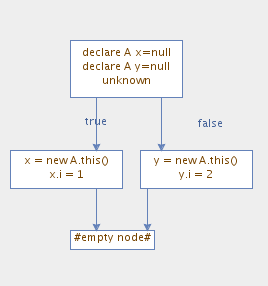
\includegraphics[width=7cm]{img/GUI_CFG.png}}
  \hspace{1cm}
  \subfloat[Heap state: Two structures\label{fig:interactiveTwo}]{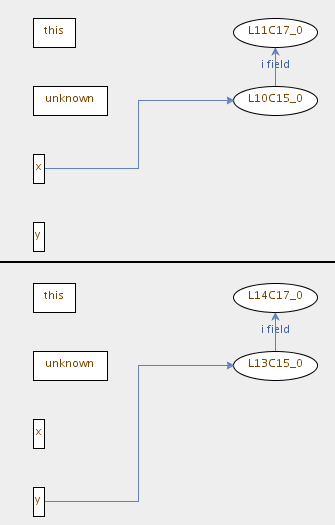
\includegraphics[width=7cm]{img/GUI_heapstate.png}}
  \hspace{0.5cm}
  \subfloat[Numerical state of heap ID\label{fig:interactiveThree}]{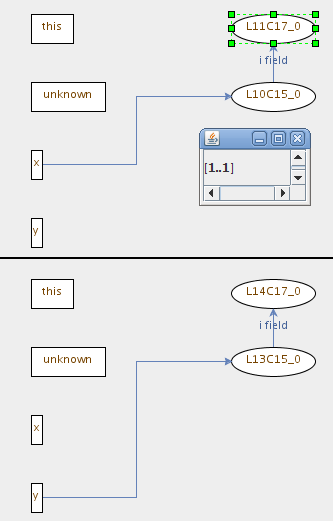
\includegraphics[width=7cm]{img/GUI_heapstateNumeric.png}}
  \caption{Sample GUI visualization}
  \label{fig:interactiveVisual}
\end{figure}

\subsubsection*{Non-interactive Visualization}
Sometimes the results of an analysis should be saved for later use in a
non-interactive fashion, such as when analyzing dozens of methods. In that case,
we generate images with graphs of all heap structures in the end state of the
program.

Automatically layouting large graphs well is a difficult endeavour, so we chose to
use \texttt{Graphviz DOT} for that task. \autoref{fig:graphvizB} shows the 
rendered graph of the heap state after executing \autoref{fig:graphvizA}. Apart
from a minor differences in appearance, the rendered graph corresponds to the
graphical notation for heaps described in \autoref{sct:notation}. That is, the program
variable \texttt{x} references the first heap node that created, namely
\texttt{L5C13\_0}, while the field \texttt{n} of the later references node
\texttt{L6C11\_0}.

\begin{figure}  
\centering
\begin{lrbox}{\mylistingbox}
\begin{minipage}[b]{.45\linewidth}
\lstinputlisting{code/graphviz.scala}
\end{minipage}
\end{lrbox}
\subfloat[Program code\label{fig:graphvizA}]{\usebox{\mylistingbox}}
\hspace{2cm}
\subfloat[Heap end
state\label{fig:graphvizB}]{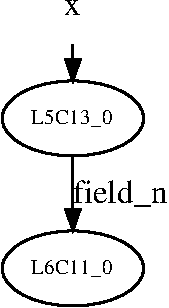
\includegraphics[scale=0.8]{img/graphvizexample-crop}}
\caption{Graphviz DOT visualization}
\label{fig:graphviz}
\end{figure}



\subsection{Performance and Optimization}
As outlined in \autoref{sct:approach}, we decided to use TVLA as an external
tool. After some experimentation it soon became evident that our analysis
suffered from severe performance problems. These were to a large part due to the
start-up of a new JVM for every call to TVLA. We then tried to invoke the
\texttt{main} method of the TVLA java library directly in order to save the
process creation and JVM initialization time which however did not work since
some static data internal to TVLA is not reset: The default binary distribution
of TVLA is designed to be used as a standalone application to analyse whole
programs, which is in sharp contrast to our use case. 

Upon request to the developers, we were able to obtain a customized version of
TVLA which allowed us to reset the internal state after one execution and then
call the \texttt{main} method again. This lead to a reduction of the execution
times of about 80\% in general.

Furthermore, we found the iteration performed by Sample to execute a program in
the abstract domain to be inefficient. While this may not be critical for other
analyses, it has a huge impact on our heap analysis. The problem is that Sample
frequently executes the same statement in the CFG several times on the same
pre-state. While the result obviously did not change, we performed a full run of
TVLA. To improve the performance, we cached the results of previous heap
operations on our heap domain: Whenever our domain is requested to perform an
operation, we check if such an operation was previously applied to the same heap
state. If that is the case, we can return the cached result. We observed a 
60\% reduction of the execution times on average. The memory usage for the caching seems to be
negligible compared to the memory footprint of TVLA.


\subsection{Testing}  
To assess the implementation of our domain, we developed two test-suites which
consist of Scala methods. We verified by manual inspection for each test case that
the results are indeed safe approximations of the real execution behaviour.

We ran Sample with two domains, our new \texttt{TVSHeap} heap domain and a
non-relational numerical domain which uses interval abstraction. All analyzed
examples are written in Scala, therefore we used the Scala compiler back-end to
translate the source code to \texttt{Simple}.

The analysis was run on a machine with a Intel Core 2 Duo at 2.53GHz and 4GB of
RAM. We used the Java HotSpot 64-Bit Server VM included in Java SE Runtime
Environment 1.6.0\_26-b03 with the option \texttt{-XX:NewRatio=2}, which helped
us to improve garbage collection performance.

\autoref{tbl:times} contains all the experimental results. Column \textbf{\#tr}
shows the number of times TVLA was called during the analysis, while column
\textbf{\#tr-unique} shows the actual calls performed when caching of the results
was enabled. The running times are displayed in columns \textbf{JVM-nc} (JVM
invocation method without caching), \textbf{JVM} (JVM with caching) and
\textbf{MR} (\texttt{main+reset} invocation method with caching).

Note that the \texttt{main+reset} invocation method produced some invalid results for the test cases \texttt{initializeFixedList}, \texttt{createNumericalList} and
\texttt{initializeAbstractedListFields}. This is most likely due to a bug in the customized
binary TVLA version that we obtained from the TVLA developers.

\begin{table}   
  \small
  \centering
  \begin{tabular}{|l|r|r|r|r|r|}
    \hline
    \textbf{Testcase} & \textbf{\# tr} & \textbf{\# tr-unique} & \textbf{JVM-nc [s] }& \textbf{JVM [s] }& \textbf{MR [s] }\\
    \hline
    \texttt{createObject} & 12 & 4 & 4.9 & 2.0 & 0.7 \\ 
    \texttt{createAndOverWrite} & 26 & 9 & 9.9 & 3.7 & 0.7 \\ 
    \texttt{assignNextField} & 26 & 9 & 10.4 & 3.9 & 0.6 \\ 
    \texttt{accessNullField} & 20 & 7 & 8.0 & 2.7 & 0.3 \\ 
    \texttt{assignFieldSelf} & 18 & 7 & 6.9 & 2.5 & 0.3 \\ 
    \texttt{overwriteField} & 24 & 10 & 8.8 & 3.8 & 0.4 \\ 
    \texttt{createObjectIfCondition} & 24 & 7 & 9.0 & 2.7 & 0.2 \\ 
    \texttt{conditionalAssignment} & 30 & 11 & 11.4 & 4.4 & 0.4 \\ 
    \texttt{conditionalAssignmentVariant} & 49 & 14 & 18.1 & 5.9 & 0.6 \\ 
    \texttt{assumeEqual} & 35 & 10 & 12.6 & 3.9 & 0.2 \\ 
    \texttt{assumeUnequal} & 32 & 13 & 11.8 & 5.1 & 0.3 \\ 
    \texttt{assumeUnequal2} & 36 & 10 & 12.7 & 3.8 & 0.2 \\ 
    \texttt{createSharedObject} & 50 & 19 & 19.8 & 8.1 & 0.8 \\ 
    \texttt{linkObjects} & 84 & 32 & 34.8 & 13.8 & 1.4 \\ 
    \texttt{linkAndTraverseObjects} & 104 & 38 & 44.2 & 16.1 & 1.9 \\ 
    \texttt{createObjectWhile} & 100 & 39 & 38.0 & 15.8 & 1.1 \\ 
    \texttt{appendByFieldAccessTwo} & 42 & 15 & 16.1 & 5.9 & 0.6 \\ 
    \texttt{buildList} & 52 & 20 & 20.1 & 7.4 & 0.5 \\ 
    \texttt{appendByFieldAccessThree} & 60 & 22 & 23.5 & 8.9 & 0.9 \\ 
    \texttt{appendByFieldAccessFour} & 112 & 72 & 116.0 & 73.6 & 4.7 \\ 
    \texttt{createPrependList} & 129 & 54 & 52.2 & 22.1 & 1.4 \\ 
    \texttt{createAppendList} & 178 & 103 & 76.7 & 47.3 & 3.3 \\ 
    \texttt{swapLoop} & 126 & 34 & 49.6 & 12.5 & 0.9 \\ 
    \texttt{accessNextSummarized} & 60 & 23 & 22.3 & 9.6 & 0.6 \\ 
    \texttt{traverseFixedShortList} & 247 & 93 & 104.0 & 48.7 & 3.3 \\ 
    \texttt{traverseSummarizedList} & 331 & 164 & 149.2 & 89.1 & 8.6 \\
    \hline
    \texttt{assignNumericField} & 22 & 8 & 9.9 & 5.0 & 1.3 \\ 
    \texttt{assignAndAccessNumericField} & 28 & 10 & 11.9 & 4.4 & 1.0 \\ 
    \texttt{createThreeElementList} & 78 & 30 & 36.2 & 13.8 & 2.0 \\ 
    \texttt{createSummarizedIntList} & 82 & 32 & 37.8 & 15.1 & 2.0 \\ 
    \texttt{assignTwoFields} & 32 & 12 & 14.8 & 5.9 & 0.9 \\ 
    \texttt{assignFieldsAndSummarize} & 112 & 44 & 58.5 & 23.6 & 4.1 \\ 
    \texttt{assignAndAddFields} & 170 & 55 & 102.2 & 32.4 & 8.3 \\ 
    \texttt{createOneOrTwoNodes} & 112 & 22 & 49.8 & 9.9 & 1.8 \\ 
    \texttt{swapHeapObjectsOnce} & 85 & 24 & 37.2 & 11.2 & 1.8 \\ 
    \texttt{initializeFixedList} & 370 & 109 & 183.8 & 57.9 &  4.5 \\ 
    \texttt{createNumericalList} & 302 & 148 & 151.7 & 79.9 & 14.4 \\ 
    \texttt{initializeAbstractedListFields} & 476 & 220 & 253.2 & 144.8 & 31.8 \\ 
    \texttt{sumListElementsZero} & 893 & 609 & 683.3 & 524.7 & 86.7 \\
    \hline
    & & & \textbf{2521.4 }& \textbf{1351.9 }& \textbf{195.4} \\
    \hline
  \end{tabular}
  \caption{Non-numerical and numerical testsuite execution times}
  \label{tbl:times}
\end{table}


\subsection{Representative  Testcases}
In this section, we present the analysis results of a few notable test cases,
representative of what we were able achieve with the new domain. Note that the
Scala code of our test cases looks rather imperative than functional because
Sample's support for interprocedural analysis is incomplete. For that reason, we
did not use any method calls.

Sometimes heap node names in the scheme we proposed tend to become too long,
so we decided to abbreviate them in the resulting graphs for the sake of
clarity. We provide the names and contents of the numerical domain separately.

\subsubsection{Multiple Structures}
Our first example in \autoref{lst:condA} illustrates how our
heap domain increases the number of three-valued structures to
represent the heap when necessary. This usually happens when previously
abstracted (summarized) parts of the heap are concretized again, and when paths
of the control flow join. Here we show the later case.   

After both branches of the \texttt{if}-statement were evaluated, we take the
least upper bound of the two states, i.e. we take the union of both structures
and move on to perform the assignment of the expression result. Canonical
abstraction determines that the structures cannot be combined into one,
since they do not agree on the value of the unary predicate for \texttt{z}. In one
structure, it points to the object referenced by \texttt{x}, while in the other
one it points to the one referenced by \texttt{y}.

It is also worth mentioning that whenever we need a condition that
cannot be determined statically, we use a boolean variable \texttt{unknown}
passed as a parameter to the method. We noticed that the Scala compiler
sometimes is smart enough to eliminate branches if conditions are too simple
(e.g. depending only on constants).

\begin{lstlisting}[float,caption={\texttt{if}-branches and heap
  structures},label={lst:condA}]
def conditionalAssignmentVariant(unknown: Boolean) = {
  val x = new A
  val y = new A
  	
  val z = if (unknown) x else y
}
\end{lstlisting}

\begin{figure}
  \begin{center}
  \begin{lrbox}{\mygraphboxA}
    \begin{tikzpicture}
    \node[hid] (n1) {n1};
    \node[var] (x) [above left=2cm and 1cm of n1] {x}
      edge [->] (n1);
    \node[var] (z) [above right=2cm and 1cm of n1] {z}
      edge [->] (n1);
    
    \node[hid] (n2) [right=3cm of n1] {n2};
    \node[var] (y) [above=of n2] {y}
      edge [->] (n2);
  \end{tikzpicture}  
\end{lrbox}
\begin{lrbox}{\mygraphboxB}
  \begin{tikzpicture}
    \node[hid] (n1) {n1};
    \node[var] (x) [above=of n1] {x}
      edge [->] (n1);
    
    \node[hid] (n2) [right=3cm of n1] {n2};
    \node[var] (y) [above left=2cm and 1cm of n2] {y}
      edge [->] (n2);
    \node[var] (z) [above right=2cm and 1 cm of n2] {z}
      edge [->] (n2);
  \end{tikzpicture}  
\end{lrbox}

  \subfloat[Structure 1]{\usebox{\mygraphboxA}}
  \hspace{3cm}
  \subfloat[Structure 2]{\usebox{\mygraphboxB}}
  
  \subfloat[Heap IDs]{\begin{tabular}{|c|c|}
    \hline
    Abbr. & Full ID  \\
    \hline
    \texttt{n1} & \texttt{L2C11\_0} \\
    \texttt{n2} & \texttt{L3C11\_0} \\
    \hline
  \end{tabular}}

  \end{center}
  \caption{Multiple Heap Structures: Result}
  \label{fig:condAssignResult}
\end{figure}


\subsubsection{Abstraction: Creation of a List} 
In the next example, things get more interesting: The program in
\autoref{lst:createPrependList} creates an unbounded number of heap objects.
More precisely, it creates a singly-linked list of one or more elements whose
head is referenced by the variable \texttt{x}. It uses a loop to allocate a new
object and prepend it to the existing tail.

Again, for technical reasons, we used the variable \texttt{unknown} to model a
condition that cannot be decided. One could also think of it as a random
variable which decided whether the (concrete) program keeps executing the loop
or stops.

It could be that the \texttt{while}-loop body is never executed: In that case, we get
a list of length one. However, if we keep executing the loop, abstraction takes
place to keep the heap bounded: All elements beyond the head are summarized into
a single one, since they look the same to TVLA (regarding the predicate values).
Therefore, a summary node is created which stands for one or more elements.

\autoref{fig:prependListResult} displays the abstract heap state after the
method was executed. It contains a structure for each of the described cases.

\begin{lstlisting}[float,caption={List creation},label={lst:createPrependList}]
def createPrependList(unknown: Boolean) = {
  var x = new A
  var t:A = null

  while (unknown) {
  	t = new A
  	t.n = x
   	x = t
	t = null
  }
}
\end{lstlisting}

\begin{figure}
  \begin{center}
  \begin{lrbox}{\mygraphboxA}
    \begin{tikzpicture}
    \node[hid] (n1) {n1};
    \node[var] (x) [above=of n1] {x}
      edge [->] (n1);
  \end{tikzpicture}  
\end{lrbox}
\begin{lrbox}{\mygraphboxB}
  \begin{tikzpicture}
    \node[hid] (n1) {n1};
    \node[var] (x) [above=of n1] {x}
      edge [->] (n1);
      
    \node[sum] (n2) [right=of n1] {n2}
    edge[<-,dashed] node[auto] {n} (n1)
    edge[->,dashed,loop] node[auto,swap] {n} (n2);

  \end{tikzpicture}  
\end{lrbox}

\subfloat[Structure 1]{\hspace{1cm}\usebox{\mygraphboxA}\hspace{1cm}}
  \hspace{3cm}
  \subfloat[Structure 2]{\usebox{\mygraphboxB}}
  
  \subfloat[Heap IDs]{\begin{tabular}{|c|c|}
    \hline
    Abbr. & Full ID  \\
    \hline
    \texttt{n1} & \texttt{L2C11\_0} \\
    \texttt{n2} & \texttt{L2C11\_0+L6C9\_0} \\
    \hline
  \end{tabular}}

  \end{center}
  \caption{Creating a list: Result}
  \label{fig:prependListResult}
\end{figure}


\subsubsection{Traversing Lists}
The last testcase showed how abstraction is performed. However, what is much
more difficult is how to obtain precise information when accessing parts
of the heap which were summarized. 

The input state at the start of the method in \autoref{lst:traverseList} consists
of a singly-linked list of length two or more. With instrumentation predicates
added (for reachability and sharing), we were able to successfully traverse the
list. We let a reference move along an arbitrary long (since abstracted) list,
pointing to the last element in the end (\autoref{fig:traverseListResult}).

This testcase also shows that our analysis actually makes use of branching
conditions: When the loop body is entered, we let the heap domain assume the
condition is true, if it is not entered we assume the negation. This can be seen
from the fact that \texttt{cur} is \texttt{null} in the end state. 

\begin{lstlisting}[float,caption={List traversal testcase},label={lst:traverseList}]
def traverseSummarizedList(x: AcyclicList) = {
  // variable which afterwards references the last element
  var end : AcyclicList = null

  var cur = x
  while (cur != null) {
    end = cur
    cur = cur.n
  } 	  
}
\end{lstlisting}

\begin{figure} 
  \begin{center}
  \begin{lrbox}{\mygraphboxA}
    \begin{tikzpicture}
    \node[hid] (n1) {n1};
    \node[var] (x) [above=of n1] {x}
      edge [->] (n1);
    \node[hid] (n2) [right=of n1] {n2}
      edge [<-] node[auto] {n} (n1);
    \node[var] (end) [above=of n2] {end}
      edge [->] (n2);
  \end{tikzpicture}  
\end{lrbox}
\begin{lrbox}{\mygraphboxB}
  \begin{tikzpicture}
    \node[hid] (n1) {n1};
    \node[var] (x) [above=of n1] {x}
      edge [->] (n1);
  
    \node[sum] (n2) [right=of n1] {n2}
    edge[<-,dashed] node[auto] {n} (n1);
    %edge[->,dashed,loop] node[auto,swap] {n} (n2);

    \node[hid] (n3) [right=of n2] {n3}
      edge [<-,dashed] node[auto] {n} (n2);
    \node[var] (end) [above=of n3] {end}
      edge [->] (n3);
  \end{tikzpicture}  
\end{lrbox}

\subfloat[Structure 1]{\hspace{1cm}\usebox{\mygraphboxA}\hspace{1cm}}
  \hspace{3cm}
  \subfloat[Structure 2]{\usebox{\mygraphboxB}}
  \hspace{3cm}

  \subfloat[Heap IDs and semantic state]{\begin{tabular}{|c|c|c|}
    \hline
    Abbr. & Full ID & Semantic Domain \\
    \hline
    \texttt{n1} & \texttt{L1C28\_0} & $\top$ \\
    \texttt{n2} & \texttt{L1C28\_1} & $\top$ \\
    \texttt{n3} & $\mathtt{(L1C28\_1)\_U1}$ & $\top$ \\
    \texttt{x} & \texttt{x} & $\top$ \\
    \texttt{end} & \texttt{end} & $\top$ \\
    \hline
  \end{tabular}}
  
  \end{center}
  \caption{Traversing a list: Result}
  \label{fig:traverseListResult}
\end{figure}

\subsubsection{Integer Fields \& Numerical Domain}
In the absence of summarization, it is desirable not to lose any precision. The
testcase in \autoref{lst:assignAdd} demonstrates that we can assign and access
fields without any precision loss since all the objects are referenced by
program variables.

We also see how the interval domain tracks the numerical information associated
with the integer-valued fields \texttt{i} and \texttt{j}. As can been seen in
\autoref{fig:assignAddResult}, in the end the sum over all fields is exactly $21$, as it
should be.

\begin{lstlisting}[float,caption={Field assignment testcase},label={lst:assignAdd}]
class TwoIntNode {
  var n: TwoIntNode = null // next
  var i: Int = 0
  var j: Int = 0
}

def assignAndAddFields = {
  val x = new TwoIntNode
  x.i = 1; x.j = 2
  var y = new TwoIntNode
  y.i = 3; y.j = 4
  var z = new TwoIntNode
  z.i = 5; z.j = 6
  x.n = y; 
  y.n = z

  val sum = x.i + x.j + x.n.i + x.n.j + x.n.n.i + x.n.n.j
}
\end{lstlisting}

\begin{figure} 
  \begin{center}
  \begin{lrbox}{\mygraphboxA}
    \begin{tikzpicture}
    \node[hid] (n1) {n1};
    \node[var] (x) [above=of n1] {x}
      edge [->] (n1);
    \node[hid] (n4) [below left=2cm and 1cm of n1] {n4}
      edge [<-] node[auto] {i} (n1);
    \node[hid] (n5) [below right=2cm and 1cm of n1] {n5}
      edge [<-] node[auto,swap] {j} (n1);
    
    \node[hid] (n2) [right=4cm of n1] {n2}
      edge [<-] node[auto] {n} (n1);
    \node[var] (y) [above=of n2] {y}
      edge [->] (n2);
     \node[hid] (n6) [below left=2cm and 1cm of n2] {n6}
      edge [<-] node[auto] {i} (n2);
    \node[hid] (n7) [below right=2cm and 1cm of n2] {n7}
      edge [<-] node[auto,swap] {j} (n2);
   
    \node[hid] (n3) [right=4cm of n2] {n3}
      edge [<-] node[auto] {n} (n2);
    \node[var] (z) [above=of n3] {z}
      edge [->] (n3);
     \node[hid] (n8) [below left=2cm and 1cm of n3] {n8}
      edge [<-] node[auto] {i} (n3);
    \node[hid] (n9) [below right=2cm and 1cm of n3] {n9}
      edge [<-] node[auto,swap] {j} (n3);
 \end{tikzpicture}  
\end{lrbox}

  \subfloat[Structure 1]{\hspace{1cm}\usebox{\mygraphboxA}\hspace{1cm}}
  \hspace{3cm}

  \subfloat[Heap IDs and semantic state]{\begin{tabular}{|c|c|c|}
    \hline
    Abbr. & Full ID & Semantic Domain \\
    \hline
    \texttt{n1} & \texttt{L8C11\_0} & $\top$ \\
    \texttt{n2} & \texttt{L10C11\_0} & $\top$ \\
    \texttt{n3} & \texttt{L12C11\_0} & $\top$ \\
    \texttt{n4} & \texttt{L9C9\_0} & $[1..1]$  \\
    \texttt{n5} & \texttt{L9C18\_0} & $[2..2]$  \\
    \texttt{n6} & \texttt{L11C9\_0} & $[3..3]$ \\
    \texttt{n7} & \texttt{L11C18\_0} & $[4..4]$ \\
    \texttt{n8} & \texttt{L13C9\_0} & $[5..5]$\\
    \texttt{n9} & \texttt{L13C18\_0} & $[6..6]$\\
    \texttt{x} & \texttt{x} & $\top$ \\
    \texttt{y} & \texttt{y} & $\top$ \\
    \texttt{z} & \texttt{z} & $\top$ \\
    \texttt{sum} & \texttt{sum} & $[21..21]$ \\
    \hline
  \end{tabular}}
  
  \end{center}
  \caption{Numerical Fields: Result}
  \label{fig:assignAddResult}
\end{figure}
\subsubsection{Replacements in Action}
We introduced the concept of replacements to update the numerical domain when
the identifiers change. Here we consider the (admittedly artificial) case where
two objects are created with integer fields of different value. The references
to these objects are then swapped depending on a condition. At the end of the
\texttt{if}-statement in \autoref{lst:swapFields}, the least upper bound of the
original and the swapped heap states is taken. While in the concrete, the
structures of these heap states are not equivalent, they look structurally the
same to TVLA: In both cases, there are two variables each pointing to a node
with an integer field. Therefore, they are joined into a single one.

Our mechanism for names is able to detect this and creates a replacement to
merge the numerical values of the fields, i.e. both fields now have the numerical
value $[1..2]$, since the distinction between the unswapped and swapped cases
was lost. The end state is depicted in \autoref{fig:swapResult}.

\begin{lstlisting}[float,caption={Swap fields testcase},label={lst:swapFields}]
def swapHeapObjectsOnce(unknown:Boolean) = {
  var x = new IntNode
  x.i = 1
  var y = new IntNode
  y.i = 2
  var t: IntNode = null
  
  if(unknown) {
    t = x
    x = y
    y = t
    t = null
  }  
}
\end{lstlisting}

\begin{figure} 
  \centering
  \subfloat[Structure 1]{
    \begin{tikzpicture}
    \node[hid] (n1) {n1};
    \node[var] (x) [above=of n1] {x}
      edge [->] (n1);
    \node[hid] (n3) [below=of n1] {n3}
      edge [<-] node[auto] {i} (n1);
    \node[hid] (n2) [right=of n1] {n2};
    \node[var] (y) [above=of n2] {y}
      edge [->] (n2);
    \node[hid] (n4) [below=of n2] {n4}
      edge [<-] node[auto] {i} (n2);
  \end{tikzpicture}}
  \hspace{1cm}
  \subfloat[Heap IDs and semantic state]{\begin{tabular}[b]{|c|c|c|}
    \hline
    Abbr. & Full ID & Semantic Domain \\
    \hline
    \texttt{n1} & \texttt{L2C11\_0+L4C11\_0} & $\top$ \\
    \texttt{n2} & \texttt{(L2C11\_0+L4C11\_0)\_U1} & $\top$ \\
    \texttt{n3} & \texttt{L3C9\_0+L5C0\_0} & $[1..2]$ \\
    \texttt{n4} & \texttt{(L3C9\_0+L5C9\_0)\_U1} & $[1..2]$ \\
    \texttt{x} & \texttt{x} & $\top$ \\
    \texttt{y} & \texttt{y} & $\top$ \\
    \hline
  \end{tabular}}
  \caption{Swapping numeric fields: Result}
  \label{fig:swapResult}
\end{figure}



\subsubsection{Initialize and Sum Lists}
In \autoref{lst:sumElements} we show the most challenging testcase we considered:
A singly-linked list is initialized with all \texttt{i} fields set to 0. We then
traverse the list and sum up all the elements we have seen and are able to
deduce that the sum is exactly 0.


\begin{lstlisting}[float,caption={Sum list elements
  testcase},label={lst:sumElements}]
def sumListElementsZero = {
  x = /* code to build and initialize a list with fields set to 0 */

  // traverse the list and sum up elements
  var cur = x
  var sum = x.i
  while (cur != null) {
    sum += cur.i
    cur = cur.n
  } 	  
}
\end{lstlisting}

\begin{figure}
  \begin{center}

    \subfloat[Structure 1]{
  \begin{tikzpicture}
  \node[hid] (n1) {n1};
  \node[var] (x) [above=of n1] {x}
    edge [->] (n1);
  \node[hid] (n3) [below=of n1] {n3}
    edge [<-] node[auto] {i} (n1);

  \node[sum] (n2) [right=3cm of n1] {n2}
    edge [<-,dashed] node[auto] {n} (n1)
    edge [->,loop,dashed] node[auto,swap] {n} (n2);
  \node[sum] (n4) [below=of n2] {n4}
    edge [<-,dashed] node[auto] {i} (n2);
  \end{tikzpicture}}
  \subfloat[Heap IDs and semantic state]{
    \begin{tabular}[b]{|c|c|c|}
    \hline
    Abbr. & Full ID & Semantic Domain \\
    \hline
    \texttt{n1} & \texttt{L194C17\_0} & $\top$ \\
    \texttt{n2} & \texttt{L196C17\_0+L198C17\_0} & $\top$ \\
    \texttt{n3} & \texttt{L195C15\_0} & $[0..0]$ \\
    \texttt{n4} & \texttt{L197C15\_0+L199C15\_0} & $[0..0]$ \\
    \texttt{x} & \texttt{x} & $\top$ \\
    \texttt{sum} & \texttt{sum} & $[0..0]$ \\
    \hline
  \end{tabular}}
  
  \end{center}
  \caption{Summing up list elements: Result}
  \label{fig:zerosumResult}
\end{figure}

\FloatBarrier

\subsection{Open Issues} 
Currently there is an open issue concerned with typing of the heap nodes: We do
not encode any type information in TVLA; i.e. all our heap nodes are untyped. It
is therefore possible that heap nodes of different type are summarized, leading
to imprecision. Instrumentation predicates could be used to consider types, but
doing so is not within the scope of this thesis, since it is a highly
non-trivial task given the complex type system of Scala.


\clearpage
\newpage
\section{Conclusions}
Our analysis yields precise results for programs that manipulate
singly-linked lists and integers, which we demonstrated in the given examples.
However, when other data structures are involved, the abstraction often becomes
imprecise very quickly. The precision may still be improved by adding more
instrumentation predicates. This would, on the other hand, degrade the
performance severely, especially when analyzing programs which do not benefit at
all from the new predicates.

We are under the impression that TVLA does not scale well to general programs.
All the examples shipped with its binary distribution contain very specific
predicates tailored towards the programs to analyze and they are not used
together.

\subsection{Future Work}

\subsection{Acknowledgements} 
I would like to thank my supervisor Dr. Pietro Ferrara for his helpful support
throughout this bachelor thesis.



\clearpage
\newpage

\bibliographystyle{alpha}
\bibliography{biblio}



\clearpage
\newpage
\begin{appendix}
\section{Detailed List of TVLA Actions}
\todo{current actions}
\lstinputlisting[language=tvp,caption={Relevant TVP actions},label=lst:tvpactions]{src/actions_basic.tvp}

%\lstinputlisting[language=tvs,caption={Test TVS},label=lst:testtvs]{src/test.tvs}

\end{appendix}
\end{document}
